\documentclass[12pt, twoside]{report}
\usepackage[TS1,T1]{fontenc}
\usepackage{lmodern}
\usepackage[utf8]{inputenc}
\usepackage{newunicodechar}
\newcommand*\longs{{\fontencoding{TS1}\selectfont s}}
\newunicodechar{ſ}{\longs}
\usepackage[a4paper,width=150mm,top=25mm,bottom=25mm,bindingoffset=6mm]{geometry}
\usepackage{enumitem}
\usepackage{amsmath}
\usepackage{float}
\usepackage{graphicx}
\usepackage{caption}
\usepackage{subcaption}
\usepackage[backend=bibtex, style=authoryear, maxcitenames=2]{biblatex}
\addbibresource{references.bib}
\usepackage{cleveref} % cleverref has to be loaded after hyperref!
\crefname{lstlisting}{listing}{listings}
\Crefname{lstlisting}{Listing}{Listings}
\usepackage{wrapfig}
\usepackage[colorinlistoftodos]{todonotes} % dont forget to remove

% listings
\usepackage{listings}
\lstset{
	captionpos=b,
	frame=single,
	breaklines=true,
	tabsize=2,
	aboveskip=4pt,
	belowskip=6pt,
	literate=%
		{Ö}{{\"O}}1
		{Ä}{{\"A}}1
		{Ü}{{\"U}}1
		{ß}{{\ss}}1
		{ü}{{\"u}}1
		{ä}{{\"a}}1
		{ö}{{\"o}}1
		{~}{{\textasciitilde}}1,
	alsoletter={{\"u}}
}
\definecolor{maroon}{rgb}{0.5,0,0}
\definecolor{darkgreen}{rgb}{0,0.5,0}
\lstdefinelanguage{XML}
{
	basicstyle=\ttfamily\footnotesize,
	morestring=[s]{"}{"},
	morecomment=[s]{?}{?},
	morecomment=[s]{!--}{--},
	commentstyle=\color{darkgreen},
	moredelim=[s][\color{black}]{>}{<},
	moredelim=[s][\color{red}]{\ }{=},
	stringstyle=\color{blue},
	identifierstyle=\color{maroon}
}

\usepackage{mdframed}
\newmdtheoremenv{defn}{Definition}[chapter]

\begin{document}

\begin{titlepage}
    \begin{center}
        \vspace*{1cm}
        
        \Huge{\textbf{Extracting recipe ingredients from cookbooks}}
        
        \vspace{1cm}
        
        \Large{by}\\
        \LARGE{Torsten Knauf}
        
        \vspace{1cm}
        
        \Large
        A thesis presented for the degree of\\
        Master of Science
        
        \vspace{1cm}
        
        
\includegraphics[width=0.4\textwidth]{Images/cau-siegel.pdf}
        
        Research Group for Communication Systems\\
        \large{at} \\
        Faculty of Engineering\\
        Christian-Albrechts-Universität zu Kiel\\
        Germany\\
        31.03.2017
    \end{center}
    
    \vspace{1cm}
    
    \LARGE
    \begin{tabbing}
    Supervisor: \= Prof. Dr.-Ing.Norbert Luttenberger\\
    \> Dr.-Ing. Jesper Zedlitz
    \end{tabbing}
\end{titlepage}

\pagenumbering{Roman}
\chapter*{Abstract}
Always do this one last, when knowing the things to praise  yourself for :P

\chapter*{Acknowledgements}
If I don't profit from nice people in these thesis, I have done something horrible wrong. So try to remember most of them here at the end... :)

\tableofcontents

\listoffigures
\begingroup
	\let\clearpage\relax
	\listoftables
\endgroup

\clearpage
\pagenumbering{arabic}  
\chapter{Introduction}
80-120Seiten anpeilen
\section{Problem-Stellung}
\section{Mein Beitrag}

A recipe parser, which can tag old and rather unstructured cookbooks according to the ontology of \parencite{schemaOrg}, is developed in this thesis. Once it is tagged, it is easy to extract the tagged entities. The parser is developed and tested with \textit{Davidis, Henriette: Praktisches Kochbuch für die gewöhnliche und feinere Küche. 4. Aufl. Bielefeld, 1849} but can be adapted easily to every German cookbook or website. For other languages new training data and dictionaries for the machine learning preparation of the parser have to be provided, but the general algorithm can be inherited.

This effort is motivated by nutritional science. Being able to extract the ingredients of a recipe automatically simplifies research according healthy food. But also sociological analysis are enabled through that.

The thesis is structured as follows:

\chapter{Motivation}

\chapter{Making a cookbook machine readable}
This chapter covers shortly, how we transform a cookbook in a machine readable format, which can be arbitrarily processed further. To achieve this, the cookbook has to be digitalised first. Afterwards it has to be enriched with meta data from an ontology.

\section{Digitalisation}
In general there are two different ways, how to digitalise a book. The first one is to scan each side and let an optical character recognition program extract the text of the scanned pictures. The second one is to type it manually into a computer.

The German Text Archive provides a collection of German texts from the 16th to the 19th century including our targeted cookbook \textit{Davidis, Henriette: Praktisches Kochbuch für die gewöhnliche und feinere Küche. 4. Aufl. Bielefeld, 1849} in \parencite{DTA}. They digitalised it through double keying, meaning that two people independent of each other manually typed the book into the computer. Differences in their versions were revised by a third person. They have already enriched the book with \textit{TEI: Text Encoding Initiative}-standard\footnote{http://www.tei-c.org/index.xml}. TEI is a standard for representing printed text in digital form. As many as possible characteristics of the printed medium are kept through meta data. Its main purpose is for analysing in humanities, social sciences and linguistics.

Because we are only interested in extracting certain data from the recipes and not in linguistic analysis or something else, we have transformed the digitalised version as depicted in \cref{fig:davidisRecipe} on the next page. The essence of this version is, that it is free of for us not relevant information like the encoding of the German \textit{\longs} and has a clear structure. 

\begin{figure}
	\begin{subfigure}{1\textwidth}
	\begin{lstlisting}[language=XML]
<div n="3">
	<head>4. Klare braune Rindflei&#x017F;ch&#x017F;uppe.</head> <lb/> <p>Die Bereitung die&#x017F;er braunen Kraftbrühe findet man in<lb/> <hi rendition="#aq">A.</hi> No. 12. Zu einer Ge&#x017F;ell&#x017F;chaft	von 12 Per&#x017F;onen nimmt<lb/> man 6 Pfund Rindflei&#x017F;ch und 1 Pfund rohen Schinken. Es<lb/> werden braune Klöße No. 3 und Schwammklöße darin gemacht.<lb/> Auch kann man nach Belieben braunen Sago darin kochen.
	</p>
</div>
	\end{lstlisting}\caption{Example recipe version from \parencite{DTA}}\vspace{1em}
	\end{subfigure}
	\begin{subfigure}{1\textwidth}
\begin{lstlisting}[language=XML]
<cue:recipe type="Suppen." rcp-id="B-4">
	<head>Klare braune Rindfleischsuppe.</head>
	
	<p>Die Bereitung dieser braunen Kraftbrühe findet man in A. No. 12. Zu einer Gesellschaft von 12 Personen nimmt man 6 Pfund Rindfleisch und 1 Pfund rohen Schinken. Es werden braune Klöße No. 3 und Schwammklöße darin gemacht. Auch kann man nach Belieben braunen Sago darin kochen.
	</p>
</cue:recipe>
\end{lstlisting}\caption{Example transformed}
	\end{subfigure}
	\caption{A recipe from our cookbook}
	\label{fig:davidisRecipe}
\end{figure}


\section{CueML ontology}\label{sec:cueMLOntology}
An ontology is needed for automatic extraction and further processing of information. In computer science an ontology is a vocabulary with defined meaning. A description for the use of ontologies can be found in \parencite{semanticWeb}.

\begin{figure}
	\begin{subfigure}{1\textwidth}
		\centering
		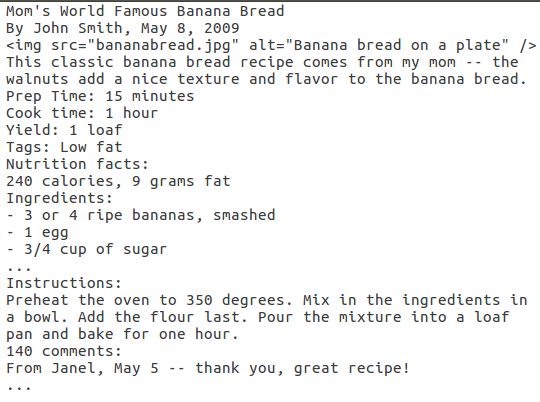
\includegraphics[width=0.7\textwidth]{Images/schemaRecipeWithoutMarkup}
		\caption{A recipe without markup}\vspace{1em}
	\end{subfigure} \\
	\begin{subfigure}{1\textwidth}
		\centering
		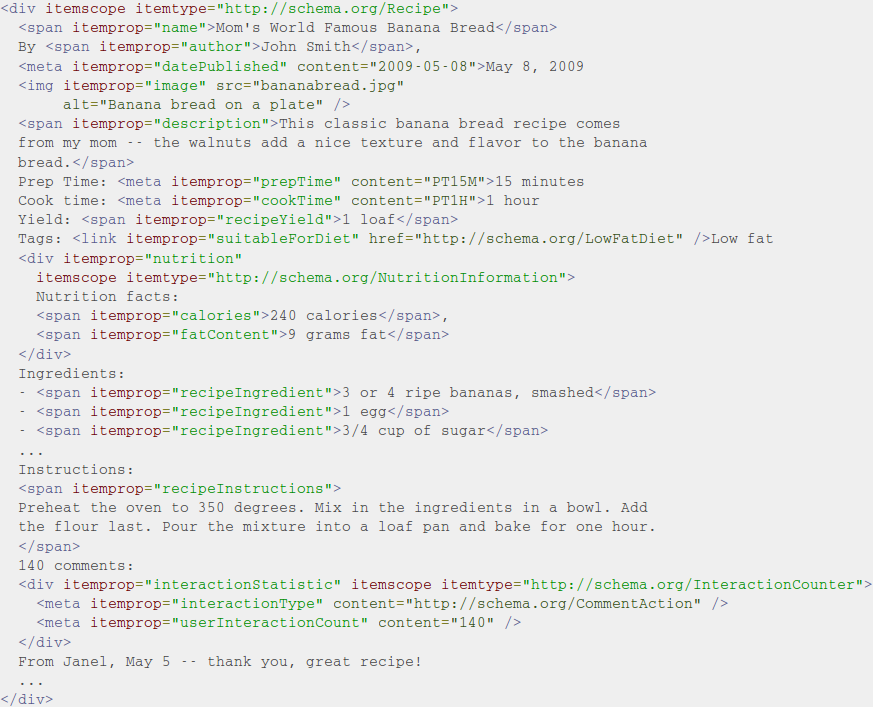
\includegraphics[width=1\textwidth]{Images/schemaRecipeWithMarkup}
		\caption{The same recipe enriched with markup}
	\end{subfigure}
	\caption{Schema.org/Recipe example from \parencite{schemaOrg}}
	\label{fig:schemaOrgRecipe}
\end{figure}

\textit{Schema.org/Recipe} is an existing ontology for recipes \parencite{schemaOrg}. For example http://cooking.nytimes.com and http://allrecipes.com use it. Its general usage is shown in \cref{fig:schemaOrgRecipe} on the next page and its main purpose is to support search engines as described in \parencite{foodBlogger} and \parencite{schemaOrg} \footnote{at http://schema.org/docs/datamodel.html}.

But it is not precise enough for further automatic culinary analysis like extracting the ingredients. As you can see in \cref{fig:schemaOrgRecipe} each line from the list of ingredients is marked as an ingredient. This is too inaccurate, because the concrete ingredient is not marked and neither its quantity nor unit. Therefore a computer cannot understand it.

That is why we came up with \textbf{culinary editions markup language (cueML)}. It is pronounced like Kümmel, which is the German word for caraway. It is an extension of Schema.org/Recipe. To extend it is a good idea, because this way it keeps all existing advantages of Schema.org/Recipe.

First of all we add the three attributes \textit{quantity}, \textit{unit} and \textit{name}. The name specifies a basis form of the ingredient. That enables a check against an external source, which for example could provide nutrition information or a category like vegetable. The markup for the recipe from \cref{fig:schemaOrgRecipe} stays the same, except that the recipeIngredient elements get these three extra attributes as shown in \cref{lst:exampleCueML}.

\begin{minipage}{\linewidth} % For avoiding page breaks
\begin{lstlisting}[language=XML, caption={Example for cueML}, label=lst:exampleCueML]
Ingredients:
- <span itemprop="recipeIngredient" quantity="3-4" name="banana">3 or 4 ripe bananas, smashed</span>
- <span itemprop="recipeIngredient" quantity="1" name="egg">1 egg</span>
- <span itemprop="recipeIngredient" quantity="0.75" unit="cup" name="sugar">3/4 cup of sugar</span>
\end{lstlisting}
\end{minipage}

Additionally we add an attribute \textit{isOptional}, because we think it is not appropriate to simply state sugar is an ingredient in the case of "sugar if not sweet enough". 

Sometimes an ingredient is composed. For example "potato dumplings" is a reference to a complete different recipe. For capturing this, we add an attribute \textit{reference}, which points to another source. We also allow an element \textit{link} with an attribute \textit{target}. This is just a look up reference for example to general cooking advice. 

Last we also noticed, that ingredients can be alternatives to each other like in "hollandaise sauce or butter, mustard and a squeeze of lemon juice". Therefore we add an element \textit{recipeIngredientAlternations} having arbitrary child elements \textit{alt}, which enclose \textit{recipeIngredient} elements.

An example is provided in \cref{appendix:fullUseOfCueML}. The complete cueML ontology is defined through a relax ng grammar, which can be found in \cref{appendix:grammaCueML}. Due to the point, that Schema.org does not provide a grammar for Schema.org/Recipe, cueML includes also the rules for it. Personally I was surprised that they do not provide an official grammar, because that would provide a clear definition as well as an easy validation method. That is why we provide a grammar. But they state themselves, that "some data is better than none", meaning, that they want to tolerate wrong meta data for reducing the risk of getting no meta data at all. They state furthermore, that it makes it more easy to extend the language \parencite{schemaOrg}\footnote{at http://schema.org/docs/datamodel.html}. Obvious you cannot break, what is not defined. 


\section{Applying cueML to our recipes}
Due to the point, that we wanted to extend Schema.org/Recipe, cueML should be applied to the list of ingredients as the former does. But our recipes have only a direction text, as you can see in \cref{fig:davidisRecipe}. CueML as well as Schema.org/Recipe is not well suited for direction text. The ingredient phrases are not always tied closely together. Besides they repeat themselves in the text and sometimes they appear in the form of "like the previous one but don't use onions". These points make it hard to apply cueML directly to the direction text. Therefore we decided to collect them in an extra \textit{meta}-element. Having extra sections for recipe yield, cook time and list of ingredients is way more nicer to read than only one direction text anyway. \Cref{appendix:fullUseOfCueML} shows a full example usage of cueML. A test with the testing tool for structured data from google\footnote{https://search.google.com/structured-data/testing-tool} reveals, that all extracting, which is already in place for Schema.org/Recipe, still works. 


\section{Need for automation}
As mentioned in \parencite{manualTagging}, manual tagging is time consuming and error prone. The approach to extract ingredients from recipes, which we will present in section \ref{sec:crfzeit}, emphasises that. They state, that they need 50-100 fields per recipe. And in the evaluation of their approach they discovered mistakes done in manual tagging.

For tagging one recipe in our cookbook I need about 5 minutes. That means, that I would need more than 2 weeks, for tagging only the recipes from our cookbook. Building a big data pool this way is very time consuming and therefore expensive.

Hence automation, which has to be configured only once and can be applied to many resources afterwards, is clearly preferable.



\chapter{Related Work}
In general there exists many works about extracting useful information from textual and unstructured resources. The superordinate term for this field of research is Text Mining. It was first mentioned in \parencite{KDT} and an overview can be found in \parencite{surveyOfTextMining}. 

The algorithms for extracting useful information depend highly on existing semi-structures, which can be taken advantage of. Here we present existing algorithms, which we found in the domain of cooking, and distinct their effort from this thesis. But before that we define precision and recall.

\section{Precision \& Recall}
NOT HERE
Precision and recall are metrics, which measure the quality of an information extracting algorithm.

\begin{equation} \label{eq:precisionAndRecall}
	Precision = \frac{\#(retrieved \cap relevant)}{\#retrieved}, \hspace{1em} Recall = \frac{\#(retrieved \cap relevant)}{\#relevant}
\end{equation}

They are defined as shown in \cref{eq:precisionAndRecall} according to  \parencite{surveyOfTextMining}. A high precision states, that the algorithm does only find relevant information as intended. The ideal precision of one would mean, that all extracted data where useful. A high recall states, that the algorithm finds many of the total relevant information. The perfect score of one would mean, that all relevant information were found. Both are needed for the evaluation of an algorithm. If only considering precision, the algorithm could only find the information, which are obvious relevant and therefore find only view information, but having a high score this way. On the other side, if only considering recall, the algorithm could return everything. This way its score would have the perfect value of one. But both algorithm are obvious not good, which gets covered by a low value of the other formula.


\section{Skip The Pizza}
\parencite{REgutGenug} is a project described on WordPress.org. The author wants to combine his two hobbies cooking and software engineering. For being able to answer questions like "How many ingredients does a typical recipe consist of?" or "Which are the most frequent ingredients?", he extracts the ingredients of recipes from an open source platform at http://recipes.wikia.com/wiki/Recipes\_Wiki.

The recipes have a consistent internal representation, which is shown in \cref{lst:recipeWiki}. The semi-structure, that after \texttt{== Ingredients ==} comes a list of ingredients, can be recognized easily. Per line is one ingredient enclosed within \texttt{[[ingredient name]]}. Using this semi-structure a regular expression is already good enough for extracting the ingredients from these recipes.

\begin{lstlisting}[frame=single, basicstyle=\footnotesize\ttfamily,caption={Shortened example recipe from \\ http://recipes.wikia.com/wiki/Recipes\_Wiki}, label=lst:recipeWiki]
* Makes 6 to 8 servings

== Ingredients ==
* 2 tbsp extra virgin [[olive oil]]
* 3 cloves [[garlic]], finely chopped
[...]

== Directions ==
Heat olive oil and garlic in large skillet over low heat until
garlic begins to sizzle.
Add tomatoes, [...]

[[Category:Cathy's Recipes]]
[[Category:Garlic Recipes]]
[...]
\end{lstlisting}


\section{Extracting Structured Data From Recipes Using Conditional Random Fields}\label{sec:crfzeit}
The New York Times provides a cooking website with recipes\footnote{http://cooking.nytimes.com/}. Their recipes are enriched with Schema.org/Recipes. For providing a recipe recommendation system based on ingredients, you have to extract the exact ingredients from a recipe, which is not enabled through this schema, as already discussed in \cref{sec:cueMLOntology}. Nevertheless they are able to extract them automatically. They use the provided structure from Schema.org/Recipe, that each ingredient phrase from the list of ingredients is marked as recipeIngredient, and Conditional Random Fields (CRF) for that. Their approach is described in \parencite{CRFZeit}. Hence we introduce here CRF first and afterwards outline their implementation.  

\subsection{Conditional Random Fields}
Given a vector of words, CRF wants to predict a suitable vector of labels. For example when the vector of words is \textit{[1 tablespoon salt]}, we want to predict \textit{[QUANTITY, UNIT, INGREDIENT]}, meaning 1 is a quantity, tablespoon a unit and salt an ingredient.

A detailed introduction to CRF can be found in \parencite{CRFIntroduction}. Here we only want to give a quick overview about linear-chain CRF, because that is the algorithm the New York Times uses. Therefore, when we write CRF, we mean linear-chain CRF.

Its starting point are vectors of words $X$, which have already correct vectors of labels $Y$. Such related sets of vectors are called training data. A joint probability distribution can be extracted from this training data, which states how likely a vector of words has a corresponding vector of labels. Taking the simplified assumption, that each label depends only on the previous label and that the current word depends only on the current label, leads to \cref{eq:jointProb}. This can always be transformed into the form of \cref{eq:magicTransoformation}. The division with $Z(X,Y)$ ensures, that the value of $p(X,Y)$ is between zero and one. $1_{condition}$ is a function, which is one if the condition is true and zero otherwise. Smart indexing leads to \cref{eq:smartIndexing}. Each $f_k$ is called a feature function. The calculation of the $\Theta_k$'s is a mathematical optimisation problem. Note that there is very likely no exact solution due to the simplified assumption of \cref{eq:jointProb}.

\begin{equation} \label{eq:jointProb}
p(X,Y) = \prod_{t=1}^T p(y_t|y_{t-1}) * p(x_t|y_t), \quad T = \#X
\end{equation}
\begin{align}\label{eq:magicTransoformation}
p(X,Y) = \frac{1}{Z(X,Y)}\prod_{t=1}^T exp(\sum_{i,j\in S}^{} \Theta_{i,j} * 1_{y_t=i} * 1_{y_{t-1}=j} + \sum_{i \in S}^{} \sum_{j \in O}^{} \mu_{o,i} * 1_{y=i} * 1_{x_t=o}), \nonumber
\\
Z(X,Y) = \sum_{X}^{}\sum_{Y}^{}\prod_{t=1}^T exp(\sum_{i,j\in S}^{} \Theta_{i,j} * 1_{y_t=i} * 1_{y_{t-1}=j} + \sum_{i \in S}^{} \sum_{j \in O}^{} \mu_{o,i} * 1_{y=i} * 1_{x_t=o}), \nonumber
\\
S = all\ possible\ labels, \quad O = all\ possible\ words
\end{align}
\begin{align} \label{eq:smartIndexing}
p(X,Y) = \frac{1}{Z(X,Y)}\prod_{t=1}^T exp(\sum_{k=1}^{K} \Theta_{k} * f_k(y_t, y_{t-1}, x_t)), \nonumber
\\
Z(X,Y) = \sum_{X,Y}^{}\prod_{t=1}^T exp(\sum_{k=1}^{K} \Theta_{k} * f_k(y_t, y_{t-1}, x_t))
\end{align}

A joint probability distribution can always be transformed into a conditional probability as shown in \cref{eq:condProb}.

\begin{equation}\label{eq:condProb}
p(Y|X) = \frac{p(X,Y)}{\sum_{Y'\in S}^{}p(Y', X)}
\end{equation}

The described model so far is a Hidden Markov Model. In a CRF you are also allowed to take only a subset of these features, what can improve performance without loosing accuracy. Additional improvement in a CRF can very likely be achieved by further custom feature functions, which may depend on the whole vector of words, instead of only the current word identity. For example some custom feature functions could be:

\begin{itemize}
\item $f_{k+1}(y_t, y_{t-1}, X) = 1_{x_t\ starts with\ upper\ case}$
\item $f_{k+2}(y_t, y_{t-1}, X) = 1_{x_t\ is\ in\ a\ domain\ specific\ dictionary}$
\item $f_{k+3}(y_t, y_{t-1}, X) = 1_{x_t\ is\ in\ a\ domain\ specific\ dictionary\ and\ x_{t-1}\ is\ an\ article}$
\end{itemize}

Putting all together leads to \cref{def:defCRF}. Note that after plugging \cref{eq:smartIndexing} into \cref{eq:condProb} $Z$ now only depends on $X$.

\begin{defn}[linear-chain Conditional Random Field] \label{def:defCRF}
    A linear-chain Conditional Random Field is a conditional distribution of the form: \vspace*{0.5em} \\
    $p(Y|X) = \frac{1}{Z(X)}\prod_{t=1}^T exp(\sum_{k=1}^{K} \Theta_{k} * f_k(y_t, y_{t-1}, X))$, where \\
    \hspace*{2em}$Z(X) = \sum_{S}^{}\prod_{t=1}^T exp(\sum_{k=1}^{K} \Theta_{k} * f_k(y_t, y_{t-1}, X))$ and \\
    \hspace*{2em}$Y$ vector of labels, $X$ vector of words, $S$ set of all possible labels
\end{defn}

Having a CRF in place, a natural prediction function is shown in \cref{eq:CRF}. The calculation of $prediction(X)$ can be done in $(\#S)^2*\#X$ through dynamic programming.

\begin{equation}\label{eq:CRF}
prediction(X) = argmax_Y(P(Y|X))
\end{equation}

\subsection{Implementation of New York Times}
As starting point the New York Times have manually specified labels for over 130,000 ingredient phrases, which they use as training data. They are extracted out of their website, where their recipes are already enriched with Schema.org/Recipe.

One example ingredient phrase is shown in \cref{lst:NYTTrainingData}. They use CRF++\footnote{https://taku910.github.io/crfpp/} as library, which is an implementation of CRF. The first word per column is the actual word. The last word is the label, which should be predicted in IOB2 format. It states, that the beginning of an entity gets prefixed with \textit{B-} and the continuation with \textit{I-}, as you can see in the last three words. Words, which do not belong to a relevant entity, get labelled with \textit{OTHER}. The labels in between are custom features. 

\begin{lstlisting}[frame=single, caption={Extract of the training data for New York Times CRF}, label=lst:NYTTrainingData]
3/4       I1  L12	 NoCAP	NoPAREN	 B-QTY
pound     I2  L12	 NoCAP	NoPAREN	 OTHER
shiitake  I3  L12	 NoCAP	NoPAREN	 B-NAME
mushrooms I4  L12	 NoCAP	NoPAREN	 I-NAME
,         I5  L12	 NoCAP	NoPAREN	 OTHER
stemmed   I6  L12	 NoCAP	NoPAREN	 B-COMMENT
and       I7  L12	 NoCAP	NoPAREN	 I-COMMENT
quartered I8  L12	 NoCAP	NoPAREN	 I-COMMENT
\end{lstlisting}

The feature functions, which the CRF should use, are not specified through functions in a concrete programming language. Instead they get described through templates of the format U00:\%x[row,column], as shown in \cref{lst:NYTfeatureTemplates}. The row specifies the targeted word in relative position to itself and the column specifies the absolute position. Therefore when the actual word is mushrooms the data from \cref{lst:NYTTrainingData} would be expended to the values in \cref{lst:NYTfeatureTemplatesDerivedValue}.

\newpage
\begin{minipage}{0.4\textwidth} 
\begin{lstlisting}[frame=single, caption={Feature templates for New York Times CRF}, label=lst:NYTfeatureTemplates]
# Unigram               
U00:%x[-2,0]             
U01:%x[-1,0]              
U02:%x[0,0]
U03:%x[1,0]
U04:%x[2,0]
U05:%x[0,1]
U06:%x[0,2]
U07:%x[0,3]

U08:%x[-2,4]
U09:%x[-1,4]
U10:%x[0,4]
U11:%x[1,4]
U12:%x[2,4]

U13:%x[0,0]/%x[0,2]
U14:%x[0,1]/%x[0,2]
U15:%x[0,0]/%x[0,3]
U16:%x[0,0]/%x[0,4]
U17:%x[0,0]/%x[0,1]

# Bigram
B
\end{lstlisting}
\end{minipage}
\hfill
\begin{minipage}{0.5\textwidth} 
\begin{lstlisting}[frame=single, caption={Derived value when the current word in \cref{lst:NYTTrainingData} is mushrooms}, label=lst:NYTfeatureTemplatesDerivedValue]
            
pound            
shiitake            
mushrooms
,
stemmed
I4
L12
NoCAP

NoPAREN
NoPAREN
NoPAREN
NoPAREN
NoPAREN

mushrooms/L12
I4/L12
mushrooms/NoCAP
mushrooms/NoPAREN
mushrooms/I4


I-NAME B-Name
\end{lstlisting}
\end{minipage}

Feature functions are extracted from these templates as shown in \cref{lst:featureFunctionExtraction}. The B-template takes the transition from $y_{t-1}$ to $y_t$ into account. Note that for example the custom feature function, if a word is inside parentheses, gets implemented through adding a label YesPAREN/NoPAREN to the trainings data in the fourth column in a preprocessing step and specifying the feature template U10\%[0,4]. Also note, that for each such template $\#(all\ possible\ labels)*\#(all\ possible\ words)$ different feature functions gets created. For the B-template $\#(all\ possible\ labels)*\#(all\ possible\ labels)*\#(all\ possible\ words)$ different feature functions gets created.

\begin{lstlisting}[frame=single, caption={Extracting of feature functions from templates}, label=lst:featureFunctionExtraction, mathescape]
U02:%[0,0]          $\rightarrow 1_{y_t=I-Name\ and\ x_t=mushrooms} $
U02:%[-2,4]         $\rightarrow 1_{y_t=I-Name\ and\ x_{t-2}\ 4th\ label\ is NoPAREN} $
U13:%x[0,0]/%x[0,2] $\rightarrow 1_{y_t=I-Name\ and\ x_t=mushrooms\ and\ x_t\ 2nd\ label\ is L12} $

B                   $\rightarrow 1_{y_t=A\ and\ y_{t-1}=B}\ for\ each\ A,B\ \in\ possible$
                                               $prediction\ labels$
\end{lstlisting}

Hence the only features the New York Times take into account for prediction are the word identity (column 0), the index of the current word (column 1), the length of the sentence (column 2, rounded to 4, 8, 12, 16 or 20), if the word starts capitalized (column 3) and if the word is inside parenthesis (column 4).

When applying their algorithm to 481 example recipes, they get 89\% sentence-level accuracy, meaning that they get 9 out of 10 ingredient phrases completely right. They tested only so few recipes, although they had over 130,000 ready labelled recipes, because they found no way for automatic evaluation. Their problem was, that there were to many ambiguous phrases and to many mistakes in the manually labelled data.
 
 
\section{Domain Specific Information Extraction for Semantic Annotation}
\parencite{GrammaBased} is a diploma thesis about extracting ingredients and their further processing from recipes. Their algorithm could be divided into two main parts.

First to check every word, if it is in a dictionary of ingredients respectively a dictionary of actions and label it accordingly. For keeping the dictionaries as small as possible they do a morphological Analysis and only store the lemmas of the words. The second main part, and more sophisticated task, is to identify, which action should be applied to which ingredient. They have a rule based approach and a dependency parsing based approach for that.

The rule based approach is to do a part of speech tagging (POS) first and afterwards try to apply a small set of rules, which define a context free grammar, with predefined meaning. \Cref{lst:ruleBased} shows an example, meaning buttermilk and bananas should be added.

\begin{lstlisting}[frame=single, basicstyle=\footnotesize\ttfamily,caption={Rule based example}, label=lst:ruleBased, mathescape]
# Example sentence
add buttermilk and bananas

# Example sentence with POS and dictionary-label
add[ACT] buttermilk[ING] and[CC] bananas[ING]

# Apply rule VP -> ACT NP (,NP)* (CC NP)?
# Predefined meaning of the rule: Apply ACT to all ING  
-> ACT NP CC NP
# Apply rule NP -> DT? JJ* ING twice  
-> ACT ING CC ING

# With: 
# VP,NP $\in$ non-terminal symbols, CC $\in$ Conjunctions, DT $\in$ Determiner, ACT := action, ING := ingredient
\end{lstlisting}

The second approach is to do a dependency based parsing, which represents the semantic structure of a sentence in a tree like format. For example \cref{fig:johnLikesApple} represents, that the subject of like is John and the liked object is Apple.
The format as well as building the tree is way more complex than the previous simple rules, but the tree can be build by already existing tools like the Stanford Parser\footnote{http://nlp.stanford.edu/software/lex-parser.shtml}. The semantic structure of the sentences give strong evidence, which action should be applied to which ingredient.

\begin{figure}[H]
	\centering
	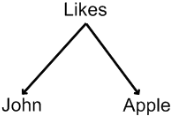
\includegraphics[]{Images/JohnLikesApple}
	\caption{John likes apple \parencite{GrammaBased}}
	\label{fig:johnLikesApple}
\end{figure}

In their evaluation they apply these two variants to 43 randomly selected recipes from the internet. Their precision and recall are presented in table \ref{tab:masterEval}. Even the more sophisticated dependency based approach has only a recall of 64\%. This is due to a lack of mapping actions to their corresponding ingredients.

\begin{table}[H]
	\centering
	\begin{tabular}{ l | c | r } 
		& Precision & Recall \\
		\hline
		Rule based & 97.39\% & 51.54\% \\
		Dependency Based & 95.4\% & 64.12\% \\
	\end{tabular}
	\caption{Evaluation Domain Specific Information Extraction for Semantic Annotation}
	\label{tab:masterEval}
\end{table}

\section{Distinction to this work}
\parencite{REgutGenug} exploits a strict semi-structure, which is not given in our very unstructured cookbook. Therefore we need more advanced algorithm than regular expressions.

\parencite{CRFZeit} take advantage of the point, that they have already marked the ingredient phrases from the list of ingredients. But our cookbook has no list of ingredients. Nevertheless, the ingredient phrases could be extracted from plain text through a CRF algorithm first and afterwards we could use the algorithm of \parencite{CRFZeit}. However we have to consider, that we do not have near as 130,000 training data. Our lack of training data could be caught up by more sophisticated custom feature functions. Maybe good feature functions even enable to extract all wanted data in one CRF algorithm.

\parencite{GrammaBased} only uses plain text. But they have a bad recall, due to the point, that they are not good in mapping actions to their corresponding ingredients. 
In contrast to mapping actions to ingredients, we want to map quantities to units and these in turn to ingredients, which is more complex and could therefore lead to an even worse recall. Though the dictionary check, enabled by a morphological analysis, from their algorithm first main part, could be very good feature functions.



\chapter{Development of recipe parser}

\section{Starting position}
-plain text
-altes deutsch / alte Zutaten
-how to test

\section{Overall picture}
Git-tag
\subsection{Workflow}
\subsection{Features}
\subsection{Evaluation}
-Precision -Recall

\section{First Iteration: Basis CRF}
Git-tag
\subsection{Workflow}
\subsection{Features}
\subsection{Evaluation}

\section{Final recipe parser}
\subsection{Workflow}
\subsection{Features}
\subsection{Evaluation}




%Discussion------------------------------------------------------------------%
\chapter{Discussion}
- Übertragung auf beliebige Bücher (Wenn Buch/Webseite hat bereits Zutatenliste erste Phase entfällt)

- TDD / früh Plausibilitäts-Überprüfungen - Tagen als Hi-Wi war ne dumme Aktion^^ (insbesondere fürs Schemata, Mengenangaben und Namen historische Recherche nötig (B-17 bzw \cref{appendix:fullUseOfCueML} cook time not clear,	Wurzelwerk, braunes Gewürz,	Engl. Soja))

- global eindeutige ids / Vokabular für Zutaten wäre nice

\section{Power of machine readable data}
Machine readable data are very powerful. But \textit{with great power comes great responsibility}\footnote{A well known proverb which probably has its origin from the French National Convention during the period of French Revolution. \parencite{quoteInvestigator}}. In the context of a recipe parser this might be a little bit exaggerated. But specially in mind of the global surveillance disclosures denounced by Edward Snowed with still uncertain dimension, I think it is important to have a consciousness for what can be done. Therefore I want to think about, what can be done through innocent looking machine readable tags. 
\bigskip

\textbf{For the good} there exists already much effort for services, which require being able to extract ingredient from recipes.

 (e.g. \cite{ingredientNetworks} or \cite{recipeRecommendation}).

Further more, having a huge machine-readable base of recipes and its ingredients, can also provide insights in sociological research. For example in \parencite{FlavorNetwork} is a comparison between American and Asian kitchen based on about 56.000 recipes.

There are many more interesting questions, which could be analysed like a historic analysis of the development and changes of cooking. Occurrences of non-local ingredients or meals are evidence for inter cultural exchange and globalisation. More expensive ingredients could be an indication for prosperity, while very simple kitchen for poverty or even wartimes.

\textbf{In the bad} \parencite{clintonHealth} "schwacher vegetarier"


\chapter{Summary}


\appendix
\chapter{Statutory Declaration}
I declare that I have developed and written the enclosed Master Thesis completely by myself, and have not used sources or means without declaration in the text. Any thoughts from others or literal quotations are clearly marked. The Master Thesis was not used in the same or in a similar version to achieve an academic grading or is being published elsewhere.
\newline
\newline
\newline
\rule{\textwidth}{1pt}
Location, Date \hfill Signature 



\chapter{Full example use of cueML} \label{appendix:fullUseOfCueML}

\begin{lstlisting}[language=XML, caption={Without cueML}]
<recipe type="Suppen." rcp-id="B-16">
	<head>Mock Turtle Suppe.</head>
	
	<p>Es wird hierzu für 24-30 Personen eine kräftige Bouillon von 8-10 Pfund Rindfleisch mit Wurzelwerk gekocht. Zugleich bringt man einen großen Kalbskopf, eine Schweineschnauze und Ohren, einen Ochsengaumen und eine geräucherte Ochsenzunge zu Feuer und kocht dies Alles gahr, aber nicht zu weich. Kalt, schneidet man es in kleine, länglich viereckige Stückchen, gibt das Fleisch in die Bouillon, nebst braunem Gewürz, ein Paar Messerspitzen Cayenne-Pfeffer, einige Kalbsmidder in Stückchen geschnitten (siehe Vorbereitungsregeln), kleine Saucissen, so viel Kalbskopfbrühe, daß man hinreichend Suppe hat, und macht dies mit in Butter braun gemachtem Mehl gebunden. Nachdem dies Alles 1/4 Stunde gekocht hat, kommen noch Klöße von Kalbfleisch, einige hart gekochte Eier in Würfel geschnitten, ein Paar Eßlöffel Engl. Soja hinzu, und wenn die Klößchen einige Minuten gekocht haben, 1/2 Flasche Madeira und auch Austern, wenn man sie haben kann. Dann wird die Suppe sogleich angerichtet.</p>
	
	<note>Anmerk. Der Soja macht die Suppe gewürzreicher, kann jedoch gut wegbleiben, und statt Madeira kann man weißen Franzwein und etwas Rum nehmen. Sowohl die Bouillon als Kalbskopf können schon am vorhergehenden Tage, ohne Nachtheil der Suppe, gekocht werden. </note>
</cue:recipe>
\end{lstlisting}


\begin{lstlisting}[language=XML, caption={Enriched with cueML}]
<div itemscope itemtype="http://schema.org/Recipe http://cueML.org">
	<recipe type="Suppen." rcp-id="B-16">
		<head><span itemprop="name">Mock Turtle Suppe</span></head>
		
		<meta>
			<span itemprop="recipeYield" quantity="24-30" unit="Personen">24-30 Personen</span>
			
			<span itemprop="recipeIngredient" name="Bouillon" reference="#Bouillon">Bouillon</span>
			<span itemprop="recipeIngredient" name="Rindfleisch" quantity="8-10" unit="Pfund">8-10 Pfund Rindfleisch</span>
			<span itemprop="recipeIngredient">Wurzelwerk</span>
			<span itemprop="recipeIngredient" name="Kalbskopf" quantity="1">1 Kalbskopf</span>
			<span itemprop="recipeIngredient" name="Schweineschnauze" quantity="1">1 Schweineschnauze</span>
			<span itemprop="recipeIngredient" name="Schweineohr">Schweineohren</span>
			<span itemprop="recipeIngredient" name="Ochsengaumen" quantity="1">1 Ochsengaumen</span>
			<span itemprop="recipeIngredient" name="Ochsenzunge" quantity="1">1 geräucherte Ochsenzunge</span>
			<span itemprop="recipeIngredient">braunes Gewürz</span>
			<span itemprop="recipeIngredient" name="Cayennepfeffer" quantity="vague" unit="Messersptize">ein Paar Messerspitzen Cayenne-Pfeffer</span>
			<span itemprop="recipeIngredient" name="Kalbsmidder" quantity="vague" reference="#A-16">einige Kalbsmidder</span>
			<span itemprop="recipeIngredient" name="Saucisson">kleine Saucissen</span>
			<span itemprop="recipeIngredient" name="Butter">Butter</span>
			<span itemprop="recipeIngredient" name="Mehl">Mehl</span>
			<span itemprop="recipeIngredient" name="Kalbfleischklöße" reference="#L-4">Klöße vom Kalbfleisch</span>
			<span itemprop="recipeIngredient" name="Ei" quantity="vague">einige hart gekochte Eier</span>
			
			<span itemprop="recipeIngredient" name="Auster" isOptional="True">Austern, wenn man sie haben kann</span>
			<span itemprop="recipeIngredient" quantity="vague" unit="EL" isOptional="True">ein Paar Eßlöffel Engl. Soja</span>
			
			<recipeIngredientAlternations>
				<alt>
					<span itemprop="recipeIngredient" name="Madeira" quantity="0.5" unit="Flasche">Madeira</span>
				</alt>
				<alt>
					<span itemprop="recipeIngredient" name="weißen Franzwein">weißen Franzwein</span>
					<span itemprop="recipeIngredient" name="Rum">etwas Rum</span>
				</alt>
			</recipeIngredientAlternations>
		</meta>

		<span itemprop="recipeInstructions">
			<p>Es wird hierzu für 24-30 Personen eine kräftige Bouillon von 8-10 Pfund Rindfleisch mit Wurzelwerk gekocht. Zugleich bringt man einen großen Kalbskopf, eine Schweineschnauze und Ohren, einen Ochsengaumen und eine geräucherte Ochsenzunge zu Feuer und kocht dies Alles gahr, aber nicht zu weich. Kalt, schneidet man es in kleine, länglich viereckige Stückchen, gibt das Fleisch in die Bouillon, nebst braunem Gewürz, ein Paar Messerspitzen Cayenne-Pfeffer, einige Kalbsmidder in Stückchen geschnitten (siehe Vorbereitungsregeln), kleine Saucissen, so viel Kalbskopfbrühe, daß man hinreichend Suppe hat, und macht dies mit in Butter braun gemachtem Mehl gebunden. Nachdem dies Alles 1/4 Stunde gekocht hat, kommen noch Klöße von Kalbfleisch, einige hart gekochte Eier in Würfel geschnitten, ein Paar Eßlöffel Engl. Soja hinzu, und wenn die Klößchen einige Minuten gekocht haben, 1/2 Flasche Madeira und auch Austern, wenn man sie haben kann. Dann wird die Suppe sogleich angerichtet. </p>

			<note>Anmerk. Der Soja macht die Suppe gewürzreicher, kann jedoch gut wegbleiben, und statt Madeira kann man weißen Franzwein und etwas Rum nehmen. Sowohl die Bouillon als Kalbskopf können schon am vorhergehenden Tage, ohne Nachtheil der Suppe, gekocht werden. </note>
		</span>
	<recipe>
</div>		
\end{lstlisting}

\chapter{RELAX NG grammar for cueML} \label{appendix:grammaCueML}


\printbibliography

\end{document}